\documentclass[a4paper]{report}
% Some basic packages
\usepackage[utf8]{inputenc}
\usepackage[T1]{fontenc}
\usepackage{textcomp}
\usepackage[english]{babel}
\usepackage{url}
\usepackage{graphicx}
\usepackage{float}
\usepackage{booktabs}
\usepackage{enumitem}

\pdfminorversion=7

% Don't indent paragraphs, leave some space between them
\usepackage{parskip}

% Hide page number when page is empty
\usepackage{emptypage}
\usepackage{subcaption}
\usepackage{multicol}
\usepackage{xcolor}

% Other font I sometimes use.
% \usepackage{cmbright}

% Math stuff
\usepackage{amsmath, amsfonts, mathtools, amsthm, amssymb}
% Fancy script capitals
\usepackage{mathrsfs}
\usepackage{cancel}
% Bold math
\usepackage{bm}
% Some shortcuts
\newcommand\N{\ensuremath{\mathbb{N}}}
\newcommand\R{\ensuremath{\mathbb{R}}}
\newcommand\Z{\ensuremath{\mathbb{Z}}}
\renewcommand\O{\ensuremath{\emptyset}}
\newcommand\Q{\ensuremath{\mathbb{Q}}}
\newcommand\C{\ensuremath{\mathbb{C}}}
\renewcommand\L{\ensuremath{\mathcal{L}}}

% Package for Petri Net drawing
\usepackage[version=0.96]{pgf}
\usepackage{tikz}
\usetikzlibrary{arrows,shapes,automata,petri}
\usepackage{tikzit}
\input{petri_nets_style.tikzstyles}

% Easily typeset systems of equations (French package)
\usepackage{systeme}

% Put x \to \infty below \lim
\let\svlim\lim\def\lim{\svlim\limits}

%Make implies and impliedby shorter
\let\implies\Rightarrow
\let\impliedby\Leftarrow
\let\iff\Leftrightarrow
\let\epsilon\varepsilon

% Add \contra symbol to denote contradiction
\usepackage{stmaryrd} % for \lightning
\newcommand\contra{\scalebox{1.5}{$\lightning$}}

% \let\phi\varphi

% Command for short corrections
% Usage: 1+1=\correct{3}{2}

\definecolor{correct}{HTML}{009900}
\newcommand\correct[2]{\ensuremath{\:}{\color{red}{#1}}\ensuremath{\to }{\color{correct}{#2}}\ensuremath{\:}}
\newcommand\green[1]{{\color{correct}{#1}}}

% horizontal rule
\newcommand\hr{
    \noindent\rule[0.5ex]{\linewidth}{0.5pt}
}

% hide parts
\newcommand\hide[1]{}

% si unitx
\usepackage{siunitx}
\sisetup{locale = FR}

% Environments
\makeatother
% For box around Definition, Theorem, \ldots
\usepackage{mdframed}
\mdfsetup{skipabove=1em,skipbelow=0em}
\theoremstyle{definition}
\newmdtheoremenv[nobreak=true]{definitie}{Definitie}
\newmdtheoremenv[nobreak=true]{eigenschap}{Eigenschap}
\newmdtheoremenv[nobreak=true]{gevolg}{Gevolg}
\newmdtheoremenv[nobreak=true]{lemma}{Lemma}
\newmdtheoremenv[nobreak=true]{propositie}{Propositie}
\newmdtheoremenv[nobreak=true]{stelling}{Stelling}
\newmdtheoremenv[nobreak=true]{wet}{Wet}
\newmdtheoremenv[nobreak=true]{postulaat}{Postulaat}
\newmdtheoremenv{conclusie}{Conclusie}
\newmdtheoremenv{toemaatje}{Toemaatje}
\newmdtheoremenv{vermoeden}{Vermoeden}
\newtheorem*{herhaling}{Herhaling}
\newtheorem*{intermezzo}{Intermezzo}
\newtheorem*{notatie}{Notatie}
\newtheorem*{observatie}{Observatie}
\newtheorem*{exe}{Exercise}
\newtheorem*{opmerking}{Opmerking}
\newtheorem*{praktisch}{Praktisch}
\newtheorem*{probleem}{Probleem}
\newtheorem*{terminologie}{Terminologie}
\newtheorem*{toepassing}{Toepassing}
\newtheorem*{uovt}{UOVT}
\newtheorem*{vb}{Voorbeeld}
\newtheorem*{vraag}{Vraag}

\newmdtheoremenv[nobreak=true]{definition}{Definition}
\newtheorem*{eg}{Example}
\newtheorem*{notation}{Notation}
\newtheorem*{previouslyseen}{As previously seen}
\newtheorem*{remark}{Remark}
\newtheorem*{note}{Note}
\newtheorem*{problem}{Problem}
\newtheorem*{observe}{Observe}
\newtheorem*{property}{Property}
\newtheorem*{intuition}{Intuition}
\newmdtheoremenv[nobreak=true]{prop}{Proposition}
\newmdtheoremenv[nobreak=true]{theorem}{Theorem}
\newmdtheoremenv[nobreak=true]{corollary}{Corollary}

% End example and intermezzo environments with a small diamond (just like proof
% environments end with a small square)
\usepackage{etoolbox}
\AtEndEnvironment{vb}{\null\hfill$\diamond$}%
\AtEndEnvironment{intermezzo}{\null\hfill$\diamond$}%
% \AtEndEnvironment{opmerking}{\null\hfill$\diamond$}%

% Fix some spacing
% http://tex.stackexchange.com/questions/22119/how-can-i-change-the-spacing-before-theorems-with-amsthm
\makeatletter
\def\thm@space@setup{%
  \thm@preskip=\parskip \thm@postskip=0pt
}


% Exercise 
% Usage:
% \exercise{5}
% \subexercise{1}
% \subexercise{2}
% \subexercise{3}
% gives
% Exercise 5
%   Exercise 5.1
%   Exercise 5.2
%   Exercise 5.3
\newcommand{\exercise}[1]{%
    \def\@exercise{#1}%
    \subsection*{Exercise #1}
}

\newcommand{\subexercise}[1]{%
    \subsubsection*{Exercise \@exercise.#1}
}


% \lecture starts a new lecture (les in dutch)
%
% Usage:
% \lecture{1}{di 12 feb 2019 16:00}{Inleiding}
%
% This adds a section heading with the number / title of the lecture and a
% margin paragraph with the date.

% I use \dateparts here to hide the year (2019). This way, I can easily parse
% the date of each lecture unambiguously while still having a human-friendly
% short format printed to the pdf.

\usepackage{xifthen}
\def\testdateparts#1{\dateparts#1\relax}
\def\dateparts#1 #2 #3 #4 #5\relax{
    \marginpar{\small\textsf{\mbox{#1 #2 #3 #5}}}
}

\def\@lecture{}%
\newcommand{\lecture}[3]{
    \ifthenelse{\isempty{#3}}{%
        \def\@lecture{Lecture #1}%
    }{%
        \def\@lecture{Lecture #1: #3}%
    }%
    \subsection*{\@lecture}
    \marginpar{\small\textsf{\mbox{#2}}}
}



% These are the fancy headers
\usepackage{fancyhdr}
\pagestyle{fancy}

% LE: left even
% RO: right odd
% CE, CO: center even, center odd
% My name for when I print my lecture notes to use for an open book exam.
% \fancyhead[LE,RO]{Gilles Castel}

\fancyhead[RO,LE]{\@lecture} % Right odd,  Left even
\fancyhead[RE,LO]{}          % Right even, Left odd

\fancyfoot[RO,LE]{\thepage}  % Right odd,  Left even
\fancyfoot[RE,LO]{}          % Right even, Left odd
\fancyfoot[C]{\leftmark}     % Center

\makeatother




% Todonotes and inline notes in fancy boxes
\usepackage{todonotes}
\usepackage{tcolorbox}

% Make boxes breakable
\tcbuselibrary{breakable}

% Verbetering is correction in Dutch
% Usage: 
% \begin{verbetering}
%     Lorem ipsum dolor sit amet, consetetur sadipscing elitr, sed diam nonumy eirmod
%     tempor invidunt ut labore et dolore magna aliquyam erat, sed diam voluptua. At
%     vero eos et accusam et justo duo dolores et ea rebum. Stet clita kasd gubergren,
%     no sea takimata sanctus est Lorem ipsum dolor sit amet.
% \end{verbetering}
\newenvironment{verbetering}{\begin{tcolorbox}[
    arc=0mm,
    colback=white,
    colframe=green!60!black,
    title=Opmerking,
    fonttitle=\sffamily,
    breakable
]}{\end{tcolorbox}}

% Noot is note in Dutch. Same as 'verbetering' but color of box is different
\newenvironment{noot}[1]{\begin{tcolorbox}[
    arc=0mm,
    colback=white,
    colframe=white!60!black,
    title=#1,
    fonttitle=\sffamily,
    breakable
]}{\end{tcolorbox}}




% Figure support as explained in my blog post.
\usepackage{import}
\usepackage{xifthen}
\usepackage{pdfpages}
\usepackage{transparent}
\newcommand{\incfig}[1]{%
    \def\svgwidth{\columnwidth}
    \import{./figures/}{#1.pdf_tex}
}

% Fix some stuff
% %http://tex.stackexchange.com/questions/76273/multiple-pdfs-with-page-group-included-in-a-single-page-warning
\pdfsuppresswarningpagegroup=1


% My name
\author{Bruno M. Pacheco}

 
\begin{document}
 
\title{Relatório 1}
\author{Bruno M. Pacheco\\
DAS 5142 - Sistemas Dinâmicos}
 
\maketitle
 
\exercise{Pêndulo Simples}

Dada a formulação apresentada na descrição do experimento para o problema do pêndulo simples, encontrou-se os pontos de equilíbrio do sistema. Por definição, sabemos que um ponto de equilíbrio $\bm{\overline{x}}$ é tal que $\bm{\dot{x}}(\bm{\overline{x}}) = 0$, assim, temos que $\dot{x_1} = x_2 = 0$ $\dot{x}_2 = 0$, portanto \[
    -a \sin x_1 = 0 \implies \sin x_1 = 0
\] o que indica que os pontos de equilíbrio do sistema são da forma $\bm{\overline{x}} = n\pi$ onde $n\in \N$. Ou seja, os pontos de equilíbrio são as posições em que o ângulo está perfeitamente equilibrado em cima do eixo ou pendurado abaixo dele.

Analisou-se, então, a estabilidade desses pontos de equilíbrio. Tem-se que \[
    J\bm{\dot{x}} = \begin{bmatrix} 0 & 1 \\ -a\cos x_1 & -b \end{bmatrix} 
. \] Primeiro, vemos claramente que, para $b=0$, os autovalores do sistema serão da forma  \[
\lambda = \pm \frac{\sqrt{-4a}}{2} = \pm \frac{i \sqrt{4a} }{2}
\], ou seja, o sistema é sempre oscilatório uma vez que $a>0$.

Para os pontos de equilíbrio da forma $\bm{\overline{x}} = (2n\pi,0)$, \[
    J\bm{\dot{x}} = \begin{bmatrix} 0 & 1 \\ -a & -b \end{bmatrix} 
\] que possui autovalores da forma \[
\lambda = \frac{-b \pm \sqrt{b^2 -4a} }{2}
\]. Assim, divide-se a análise em dois casos. O primeiro, caracterizado por autovalores reais:
\begin{align*}
    &a < \left(\frac{b}{2}\right)^2 \\
    &\implies \sqrt{b^2 - 4a} \in \R \\
    &\implies \mathcal{R}(\lambda) = \frac{-b\pm\sqrt{b^2 - 4a} }{2}
\end{align*}
assim, analisamos cada um dos dois autovalores. Neste caso, claramente\[
    \lambda_2 = \frac{-b - \sqrt{b^2 -4a} }{2} < 0
\]. Em relação ao outro autovalor, tem-se que 
\begin{align*}
    &\lambda_2 = \frac{-b + \sqrt{b^2 -4a} }{2} \\
    &-b = -\sqrt{b^2} < -\sqrt{b^2-4a} \\
    &\implies -b + \sqrt{b^2 -4a} < -\sqrt{b^2-4a} + \sqrt{b^2-4a} \\
    &\implies \lambda_2 < 0 \\
.\end{align*}

Já no outro caso 
\begin{align*}
    &a \ge  \left(\frac{b}{2}\right)^2 \\
    &\implies \mathcal{R}(\lambda) = \frac{-b}{2} < 0
.\end{align*}
Portanto, sabemos que os autovalores estão sempre no semiplano esquerdo, o que nos garante que o sistema nos pontos de equilíbrio da forma $\bm{\overline{x}} = 2n\pi$ é estável.

Agora, para os pontos de equilíbrio da forma $\bm{\overline{x}} = (2n+1)\pi$ tem-se \[
    J\bm{\dot{x}} = \begin{bmatrix} 0 & 1 \\ a & -b \end{bmatrix} 
\] e, portanto, tem autovalores \[
\lambda = \frac{-b \pm \sqrt{b^2 +4a} }{2}
\]. Entretanto, $\sqrt{b^2 +4a} >  b$, portanto \[
    \lambda_2 = \frac{-b - \sqrt{b^2 -4a} }{2} <  0
\] e \[
    \lambda_1 = \frac{-b + \sqrt{b^2 -4a} }{2} <  0
\], ou seja, estes pontos de equilíbrio são instáveis.

Simulou-se, então, o sistema do pêndulo simples utilizando o aplicativo \emph{pplane8} no MATLAB. Para a configuração de parâmetros $a=1, b=0$, o aplicativo foi configurado da forma ilustrada na figura \ref{fig:figures-pplane_pendulo_simples_1-png}.

\begin{figure}[h]
    \centering
    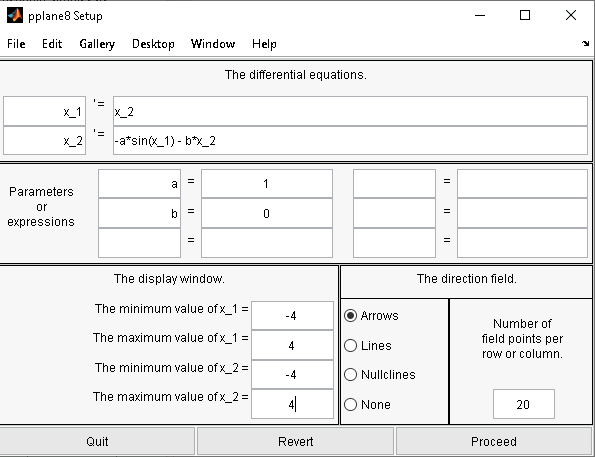
\includegraphics[width=0.6\textwidth]{figures/pplane_pendulo_simples_1.png}
    \caption{Configuração do sistema do pêndulo simples no aplicativo pplane8.}
    \label{fig:figures-pplane_pendulo_simples_1-png}
\end{figure}

O resultado da simulação pode ser observado na figura \ref{fig:figures-pplane_pendulo_simples_2-png}. Vemos que, sem atrito, o sistema conserva sua energia, alternando entre cinética e gravitacional, para qualquer estado inicial que não seja o equilíbrio. Ainda mais, pode-se observar dois movimentos possíveis para o pêndulo: um oscilatório marcado pelas trajetórias fechadas, quando a sua energia cinética não é o suficiente para que ele complete uma volta e portanto sua velocidade angular alterna o sinal periodicamente; e um rotativo marcado pelas trajetórias abertas nas extremidades verticais do gráfico, em que sua energia cinética inicial é suficiente para que ele complete uma volta e, portanto, não tenha uma inversão na direção da sua velocidade angular. Nota-se que a modelagem faz com que o segundo tipo de movimento detectado não aparente ser um ciclo limite, uma vez que a posição angular foi modelada em um espaço cartesiano ("não cíclico"). Entretanto, a interpretação física do problema nos permite apontar que esse também representa trajetórias fechadas.

\begin{figure}[h]
    \centering
    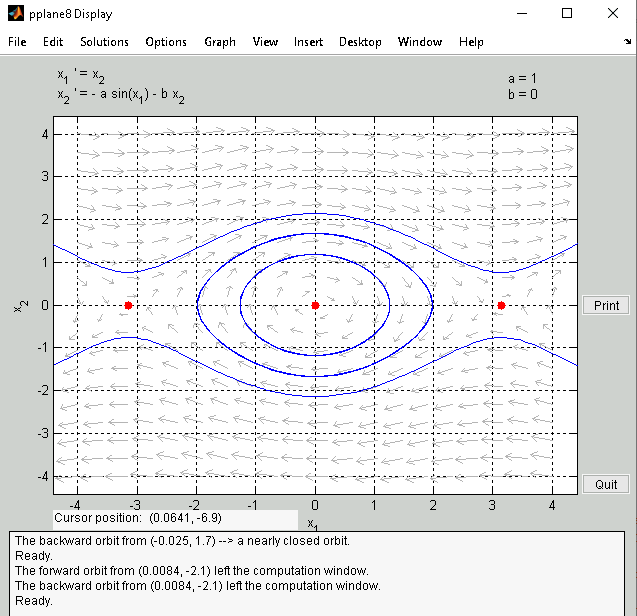
\includegraphics[width=0.6\textwidth]{figures/pplane_pendulo_simples_2.png}
    \caption{Espaço de estados do modelo do pêndulo simples sem atrito. Em vermelho marcam-se os pontos de equilíbrio e em azul possíveis trajetórias do estado.}
    \label{fig:figures-pplane_pendulo_simples_2-png}
\end{figure}

Simula-se, após, o sistema com a adição do atrito ($b=0.1$). O resultado é visível na figura \ref{fig:figures-pplane_pendulo_simples_3-png}. Observamos agora que o sistema se torna estável, com suas trajetórias convergindo para o ponto de equilíbrio em $(0,0)$, tal qual calculado.

\begin{figure}[H]
    \centering
    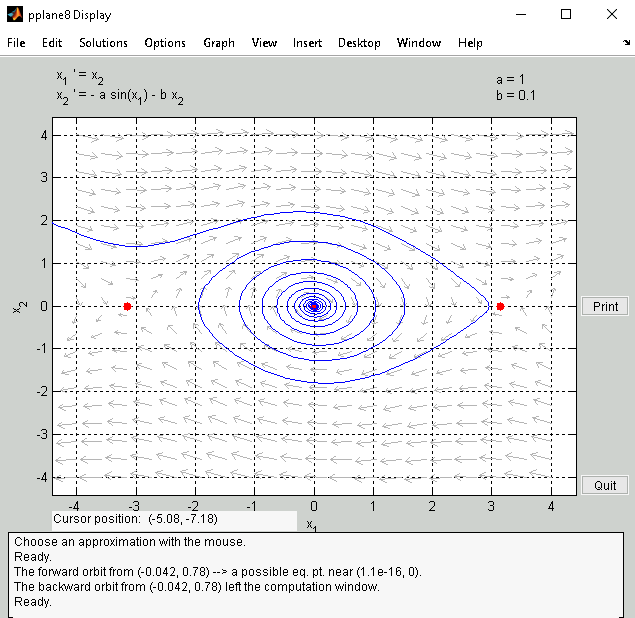
\includegraphics[width=0.6\textwidth]{figures/pplane_pendulo_simples_3.png}
    \caption{Espaço de estados do modelo do pêndulo simples com atrito.}
    \label{fig:figures-pplane_pendulo_simples_3-png}
\end{figure}

Para verificar as reações do sistema no domínio do tempo implementou-se o modelo conforme visível na figura \ref{fig:figures-simulink_pendulo_simples_1-png}. Os resultados da simulação podem ser observados na figura \ref{fig:figures-simulink_pendulo_simples_2-png}. Vê-se que os resultados são consistentes com a análise feita.

\begin{figure}[H]
    \centering
    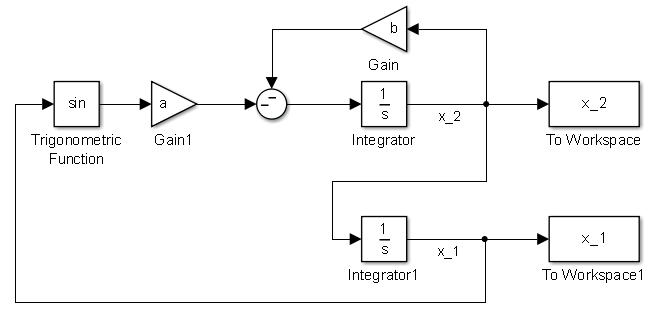
\includegraphics[width=0.6\textwidth]{figures/simulink_pendulo_simples_1.png}
    \caption{Modelo do pêndulo simples implementado no Simulink.}
    \label{fig:figures-simulink_pendulo_simples_1-png}
\end{figure}

\begin{figure}[H]
    \centering
    \begin{subfigure}{0.45\textwidth}
	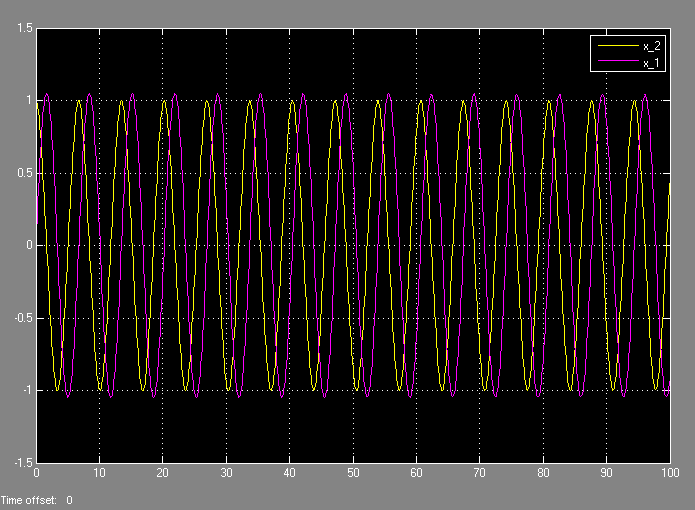
\includegraphics[width=\textwidth]{figures/simulink_pendulo_simples_2.png}
	\caption{$a=1$ e $b=0$, estado inicial $(0,1)$.}
    \end{subfigure}
    \begin{subfigure}{0.45\textwidth}
	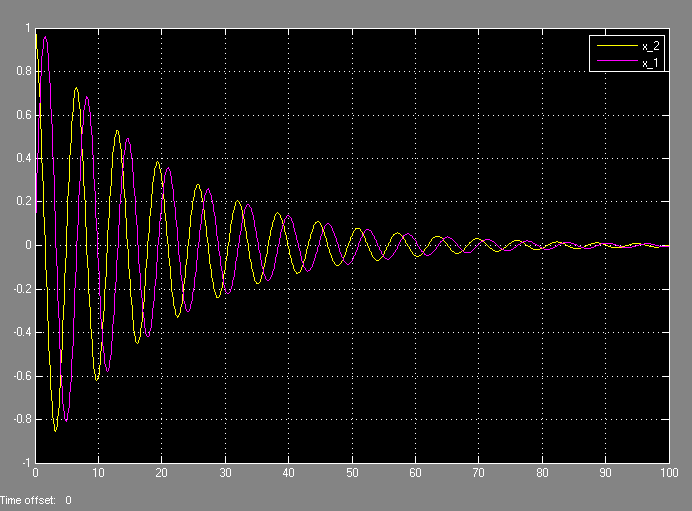
\includegraphics[width=\textwidth]{figures/simulink_pendulo_simples_3.png}
	\caption{$a=1$ e $b=0.1$, estado inicial $(0,1)$.}
    \end{subfigure}
    \caption{Simulação do modelo do pêndulo simples com diferentes parâmetros, ambos com estado inicial $(0,0)$.}
    \label{fig:figures-simulink_pendulo_simples_2-png}
\end{figure}

\exercise{Oscilador de Van der Pol (VDP)}

O sistema fornecido foi modelado através de duas variáveis de estado: $x_1(t)=x(t)$ e $x_2(t)=\dot{x}(t)$. Assim, o modelo do sistema utilizado torna-se \[
    \begin{cases}
        \dot{x}_1(t) = x_2(t) \\
	\dot{x}_2(t) = -\mu\left( x_1(t)^2 - 1 \right) x_2(t) - x_1(t)
    \end{cases}
\]. Primeiro nota-se que o ponto de equilíbrio do sistema independe do parâmetro $\mu$ e é sempre $\bm{\overline{x}}=(0,0)$.

Assim, estudou-se o comportamento do sistema de acordo com os valores do parâmetro $\mu$.

\subsection*{$\mu = 0$}

Neste caso, o sistema torna-se \[
    \begin{cases}
        \dot{x}_1(t) = x_2(t) \\
	\dot{x}_2(t) = - x_1(t)
    \end{cases}
\]. A matriz jacobiana do sistema \[
\begin{bmatrix} 0 & 1 \\ -1 & 0 \end{bmatrix} 
\] tem autovalores $\lambda = \pm i$, o que nos indica que o sistema em torno do ponto de equilíbrio é conservativo, tendo comportamento oscilatório.

Verificou-se o comportamento do sistema através do aplicativo \emph{pplane8}. O resultado é visível na figura \ref{fig:figures-pplane_vdp_1}. Novamente, vemos o caráter oscilatório do sistema tanto na trajetória presente no espaço de estados quanto no diagrama dos estados no tempo.

\begin{figure}[H]
    \centering
    \begin{subfigure}{0.45\textwidth}
	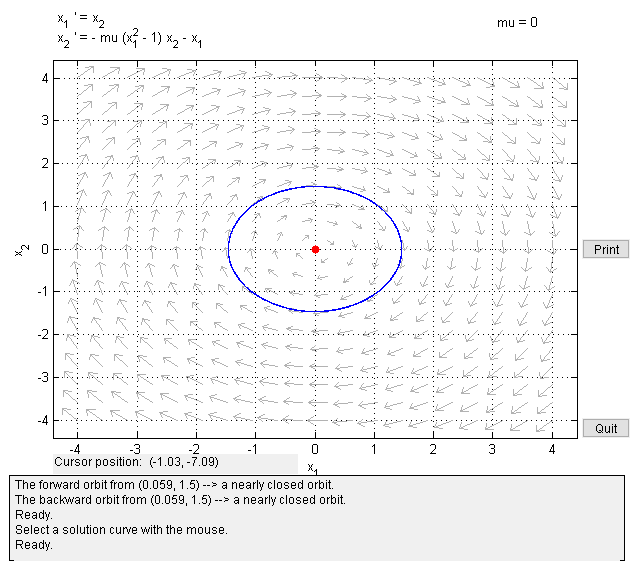
\includegraphics[width=\textwidth]{figures/pplane_vdp_1_1.png}
	\caption{Espaço de estados do sistema.}
    \end{subfigure}
    \begin{subfigure}{0.45\textwidth}
	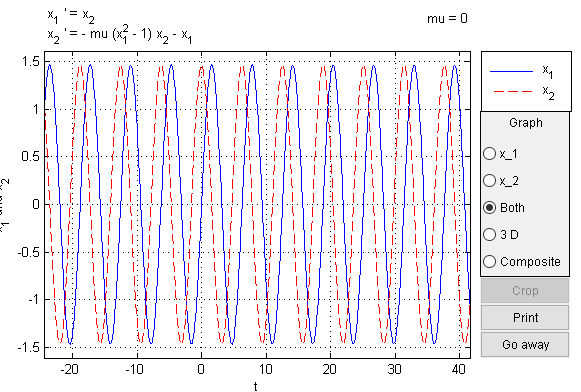
\includegraphics[width=\textwidth]{figures/pplane_vdp_1_2.png}
	\caption{Resposta do sistema (estados) no tempo.}
    \end{subfigure}
    \caption{Resposta do oscilador de Van der Pol com $\mu=0$.}
    \label{fig:figures-pplane_vdp_1}
\end{figure}

\subsection*{$\mu<0$}

Neste caso, a matriz jacobiana do sistema \[
    \begin{bmatrix} 0 & 1 \\ -1-2\mu x_1x_2 & -\mu (x_1^2-1) \end{bmatrix} 
\] avaliada no ponto de equilíbrio apresenta autovalores \[
    \lambda = \frac{\mu \pm \sqrt{\mu^2 - 4} }{2}
\]. Para $\mu \ge  -2$, temos que $\mathcal{R}(\lambda) = \frac{\mu}{2}$. Agora para $\mu > 2$, temos que $|\mu| = |\sqrt{\mu^2}| > |\sqrt{\mu^2 - 4}|$, portanto, $\lambda < 0$. Assim, conclui-se que o sistema é estável no ponto de equilíbrio. A verificação dessas conclusões pode ser observada no resultado da simulação visível na figura \ref{fig:figures-pplane_vdp_2}.

\begin{figure}[H]
    \centering
    \begin{subfigure}{0.45\textwidth}
	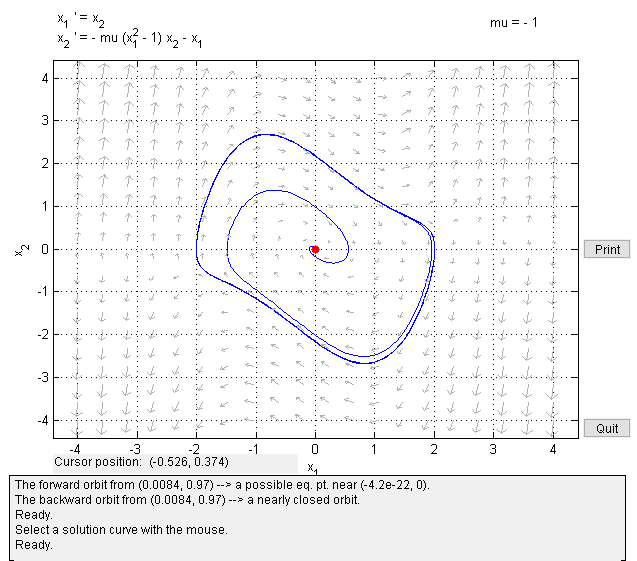
\includegraphics[width=\textwidth]{figures/pplane_vdp_2_1.png}
	\caption{Espaço de estados do sistema.}
    \end{subfigure}
    \begin{subfigure}{0.45\textwidth}
	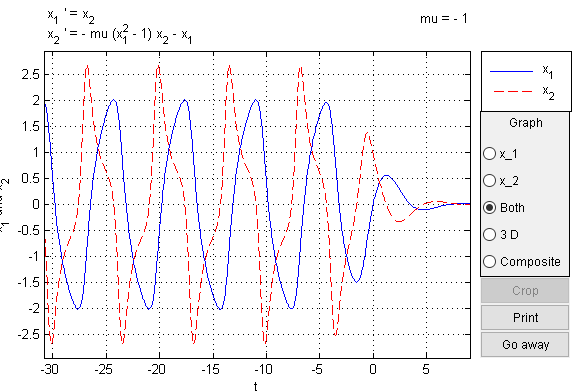
\includegraphics[width=\textwidth]{figures/pplane_vdp_2_2.png}
	\caption{Resposta do sistema (estados) no tempo.}
    \end{subfigure}
    \caption{Resposta do oscilador de Van der Pol com $\mu=-1$.}
    \label{fig:figures-pplane_vdp_2}
\end{figure}

\subsection*{$\mu>0$}

Similar ao caso anterior, entretanto agora temos os autovalores do sistema sempre positivos, concluindo, então, que o ponto de equilíbrio é instável. A resposta simulada do sistema pode ser observada na figura \ref{}. Observa-se que, mesmo começando nas imediações do ponto de equilíbrio, os estados entram rapidamente em uma trajetória oscilatória limitada, ou seja, o valor dos estados mantém-se limitados. Além disso, é evidente também a simetria entre as trajetórias oscilatórias deste com o caso anterior.

\begin{figure}[H]
    \centering
    \begin{subfigure}{0.45\textwidth}
	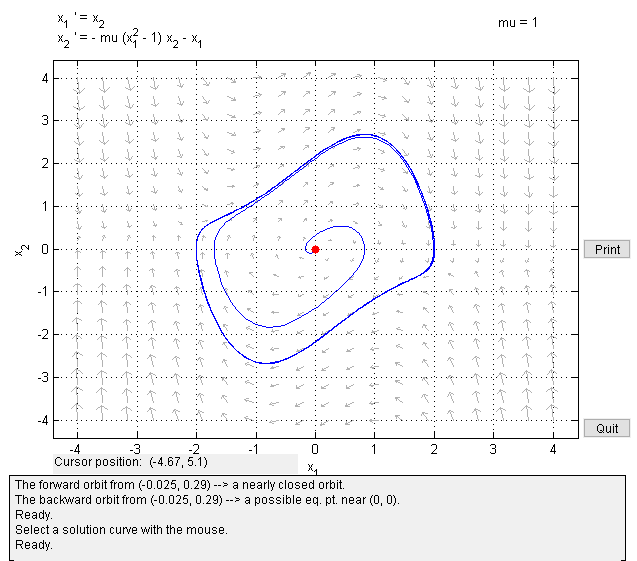
\includegraphics[width=\textwidth]{figures/pplane_vdp_3_1.png}
	\caption{Espaço de estados do sistema.}
    \end{subfigure}
    \begin{subfigure}{0.45\textwidth}
	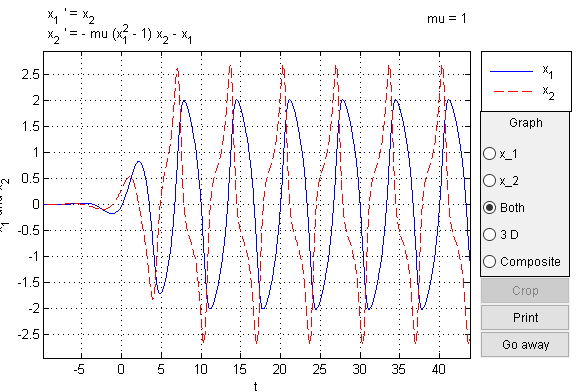
\includegraphics[width=\textwidth]{figures/pplane_vdp_3_2.png}
	\caption{Resposta do sistema (estados) no tempo.}
    \end{subfigure}
    \caption{Resposta do oscilador de Van der Pol com $\mu=1$.}
    \label{fig:figures-pplane_vdp_2}
\end{figure}

\end{document}
